%% ============================================================ 3 DISCRETE RANDOM VARIABLES
\clearpage
\inchap{Discrete Random Variables}
\section{Probability Distribution}
\begin{center}\bba\small
\begin{tabular}{|M{3.6cm}|M{6.2cm}|L{5.4cm}|}\hline
\textbf{Item} & \textbf{Result} & \textbf{Note}\\\Xhline{2pt}
Discrete r.v.\ $X$ & takes separate values $x_1,x_2,\dots$ (counts) & e.g.\ number of heads\\\hline
Probability distribution & table of $x$ against $\Pp{X=x}$ & \\\hline
Conditions & $0\leqslant\Pp{X=x}\leqslant1$ \ \ and \ \ $\displaystyle\sum_{\text{all }x}\Pp{X=x}=1$ & use to find an unknown constant\\\hline
\end{tabular}\end{center}
\noindent\begin{minipage}[c]{0.58\textwidth}
\centering\ba\small
\begin{tabular}{|c|c|c|c|c|}\hline
$x$&1&2&3&4\\\hline
$\Pp{X=x}$&$k$&$2k$&$3k$&$4k$\\\hline
\end{tabular}
\cdisp{\sum\Pp{X=x}&=1\\10k&=1\\\therefore\ k&=0.1}
\end{minipage}\hfill
\begin{minipage}[c]{0.38\textwidth}
\centering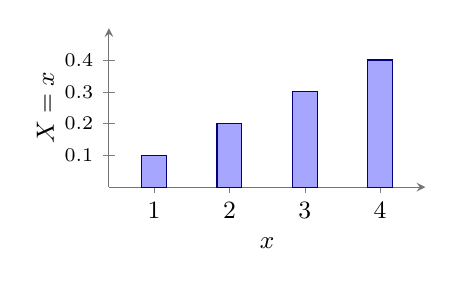
\begin{tikzpicture}
\begin{axis}[ybar,width=5.6cm,height=3.6cm,bar width=9pt,ymin=0,ymax=0.5,xmin=0.4,xmax=4.6,clip=false,xtick={1,2,3,4},ytick={0.1,0.2,0.3,0.4},yticklabel style={font=\scriptsize},xticklabel style={font=\small},axis lines=left,axis line style={thin,black!55},xlabel={$x$},ylabel={$\Pp{X=x}$},label style={font=\small},ylabel style={yshift=-3pt}]
\addplot[fill=blue!35,draw=blue!50!black] coordinates{(1,0.1)(2,0.2)(3,0.3)(4,0.4)};
\end{axis}\end{tikzpicture}
\end{minipage}
\section{Expectation and Variance}
\begin{center}\bba\small
\begin{tabular}{|M{4.4cm}|M{6.4cm}|L{4.4cm}|}\hline
\textbf{Result} & \textbf{Formula} & \textbf{Note}\\\Xhline{2pt}
Expectation (mean) & $\E(X)=\mu=\displaystyle\sum x\,\Pp{X=x}$ & long-run average\\\hline
Expectation of a function & $\E(g(X))=\displaystyle\sum g(x)\,\Pp{X=x}$ & e.g.\ $\E(X^{2})=\sum x^{2}\Pp{X=x}$\\\hline
Variance & $\Var(X)=\E\!\left[(X-\mu)^{2}\right]=\E(X^{2})-\left[\E(X)\right]^{2}$ & $\Var(X)\geqslant0$\\\hline
Standard deviation & $\sigma=\sqrt{\Var(X)}$ & \\\hline
\end{tabular}\end{center}
\gcs{enter $x$ in \gc{L1}, $\Pp{X=x}$ in \gc{L2}. \gckey{STAT} $\to$ \gc{CALC} $\to$ \gc{1-Var Stats} \ \gc{L1,L2}. Then \ \gc{$\bar{x}$}$=\E(X)$, \ \gc{$\sigma$x}$=\sigma$ (not \gc{Sx}); $\Var(X)=\sigma^{2}$. \ $\E(X^{2})=\Var(X)+[\E(X)]^{2}$, or read \gc{$\Sigma$x$^{2}$}.}
\cdisp{\E(X)&=1(0.1)+2(0.2)+3(0.3)+4(0.4)=3\\\E(X^{2})&=1(0.1)+4(0.2)+9(0.3)+16(0.4)=10\\\Var(X)&=10-3^{2}=1}
\section{Linear Functions and Combinations}
\begin{center}\renewcommand{\arraystretch}{1.05}\small
\begin{tabular}{|M{4.0cm}|M{5.6cm}|L{5.6cm}|}\hline
\textbf{Result} & \textbf{Formula} & \textbf{Condition}\\\Xhline{2pt}
Linear function & $\E(aX+b)=a\E(X)+b$ & always\\\hline
 & $\Var(aX+b)=a^{2}\Var(X)$ & always; $b$ does not change spread\\\hline
Sum / difference & $\E(aX\pm bY)=a\E(X)\pm b\E(Y)$ & always\\\hline
 & $\Var(aX\pm bY)=a^{2}\Var(X)+b^{2}\Var(Y)$ & $X$, $Y$ \textbf{independent}; variances \textbf{add} for $\pm$\\\hline
Sum of $n$ observations & $\E(X_{1}+X_{2}+\cdots+X_{n})=n\mu$ & always (independence not needed)\\\hline
 & $\Var(X_{1}+X_{2}+\cdots+X_{n})=n\sigma^{2}$ & $X_{1},\dots,X_{n}$ \textbf{independent} observations of $X$\\\hline
One observation $\times\,n$ & $\E(nX)=n\mu$ & always\\\hline
 & $\Var(nX)=n^{2}\sigma^{2}$ & always; $\Var(nX)\neq\Var(X_{1}+\cdots+X_{n})$\\\hline
\end{tabular}\end{center}
\Needspace{8\baselineskip}
\noindent\begin{minipage}[t]{0.48\textwidth}
\exlab $Y=3X-2$, using $\E(X)=3$, $\Var(X)=1$
\cdisp{\E(Y)&=3(3)-2=7\\\Var(Y)&=3^{2}(1)=9}
\end{minipage}\hfill
\begin{minipage}[t]{0.48\textwidth}
\exlab Prize $W$: $0,4,10$ with probabilities $0.6,0.3,0.1$; cost to play $\$3$
\cdisp{\E(W)&=0+1.2+1=2.2\\\E(\text{gain})&=2.2-3=-0.8\\\therefore\ &\text{not a fair game}}
\end{minipage}
\begin{info}[title=Note]
\begin{itemize}\setlength{\itemsep}{0pt}
\item If a game is \textbf{fair}, $\E(\text{gain})=0$.
\item To find the expected value of a variable other than the original $X$, there are two options:
\begin{enumerate}[label=(\arabic*),nosep]
\item link the new variable to the old one, e.g.\ $Y=5-2X$, then apply the expectation formulas;
\item draw an entirely new table for the new variable and find the expectation directly from that table.
\end{enumerate}
\end{itemize}
\end{info}
